% Capítulo 11: fila circular de 5 posições depois de a volta acontecer.
\documentclass[border=4pt]{standalone}
\usepackage[utf8]{inputenc}
\usepackage[T1]{fontenc}
% Estilo comum das figuras de vetores (capítulo 8).
\usepackage{tikz}
\usetikzlibrary{arrows.meta, positioning, calc, decorations.pathreplacing}
\definecolor{navy}{RGB}{23,45,80}
\definecolor{laranja}{RGB}{250,110,29}
\definecolor{cinzalogo}{RGB}{107,114,126}
\definecolor{azul}{RGB}{205,222,247}
\tikzset{
  casa/.style={draw=navy, line width=0.9pt, minimum width=8mm, minimum height=7mm,
               inner sep=0pt, font=\sffamily\small},
  pronta/.style={casa, fill=azul},
  parte/.style={casa, fill=laranja!12},
  marcada/.style={casa, fill=laranja!45, draw=laranja},
  fora/.style={casa, draw=cinzalogo!60, dashed, fill=white, text=cinzalogo!60},
  indice/.style={font=\sffamily\scriptsize, text=cinzalogo},
  explica/.style={font=\sffamily\small, text=navy, anchor=east},
  legenda/.style={font=\sffamily\scriptsize, text=cinzalogo},
  rotulo/.style={font=\sffamily\small\bfseries, text=navy},
  seta/.style={-{Stealth[length=2.2mm]}, navy, line width=0.9pt},
  chave/.style={decorate, decoration={brace, amplitude=4pt, mirror}, navy, line width=0.8pt},
}
% \vetor{nome}{x}{y}{valor/estilo, valor/estilo, ...}: casas lado a lado, chamadas nome0, nome1...
\newcommand{\vetor}[4]{%
  \foreach \valor/\estilo [count=\i from 0] in {#4} {
    \node[\estilo] (#1\i) at ($(#2, #3) + (\i*0.8, 0)$) {\valor};
  }
}

\tikzset{
  casa/.append style={minimum width=12mm, minimum height=8mm},
  ordem/.style={font=\sffamily\scriptsize\bfseries, text=laranja},
}
\begin{document}
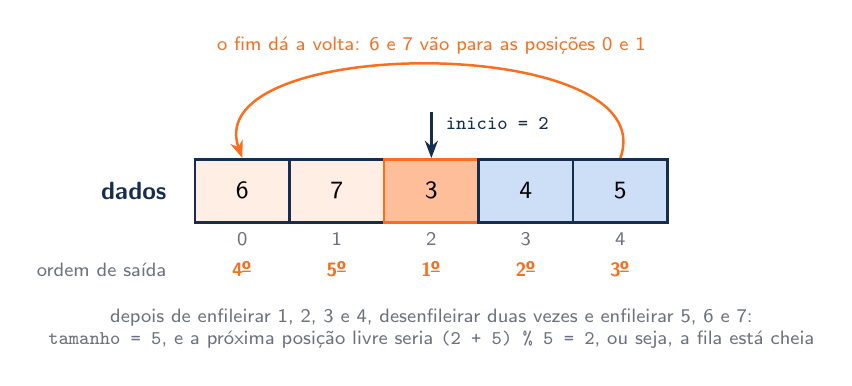
\begin{tikzpicture}[x=12mm]
  \foreach \v/\e [count=\i from 0] in {6/parte, 7/parte, 3/marcada, 4/pronta, 5/pronta} {
    \node[\e] (c\i) at (\i, 0) {\v};
    \node[indice] at (\i, -0.62) {\i};
  }
  \node[rotulo, anchor=east] at (-0.7, 0) {dados};
  \draw[seta] (2, 1.0) -- (c2.north);
  \node[legenda, text=navy, anchor=west] at (2.05, 0.85) {\texttt{inicio = 2}};
  \draw[seta, laranja] (c4.north) to[out=70, in=110, looseness=0.9] node[above, legenda, text=laranja] {o fim dá a volta: 6 e 7 vão para as posições 0 e 1} (c0.north);
  \foreach \i/\o in {2/1, 3/2, 4/3, 0/4, 1/5} {
    \node[ordem] at (\i, -1.0) {\o\textordmasculine};
  }
  \node[legenda, anchor=east] at (-0.7, -1.0) {ordem de saída};
  \node[legenda, align=center] at (2, -1.75) {depois de enfileirar 1, 2, 3 e 4, desenfileirar duas vezes e enfileirar 5, 6 e 7:\\\texttt{tamanho = 5}, e a próxima posição livre seria \texttt{(2 + 5) \% 5 = 2}, ou seja, a fila está cheia};
\end{tikzpicture}
\end{document}
